\chapter{\ifproject%
\ifcpe โครงสร้างและขั้นตอนการทำงาน\else Project Structure and Methodology\fi
\else%
\ifcpe โครงสร้างของโครงงาน\else Project Structure\fi
\fi
}

% ในบทนี้จะกล่าวถึงหลักการ และการออกแบบระบบ

\makeatletter

% \renewcommand\section{\@startsection {section}{1}{\z@}%
%                                    {13.5ex \@plus -1ex \@minus -.2ex}%
%                                    {2.3ex \@plus.2ex}%
%                                    {\normalfont\large\bfseries}}

\makeatother
%\vspace{2ex}
% \titleformat{\section}{\normalfont\bfseries}{\thesection}{1em}{}
% \titlespacing*{\section}{0pt}{10ex}{0pt}

\section{Model View Controller (MVC)}
โครงงานนี้ใช้ design pattern MVC~\cite{mvc}\CIreply{ทำไมเป็นคำว่า ``และ''}แบ่งออกเป็น 3 ส่วนหลักๆ คือ model, view และ controller
\begin{figure}
\begin{center}
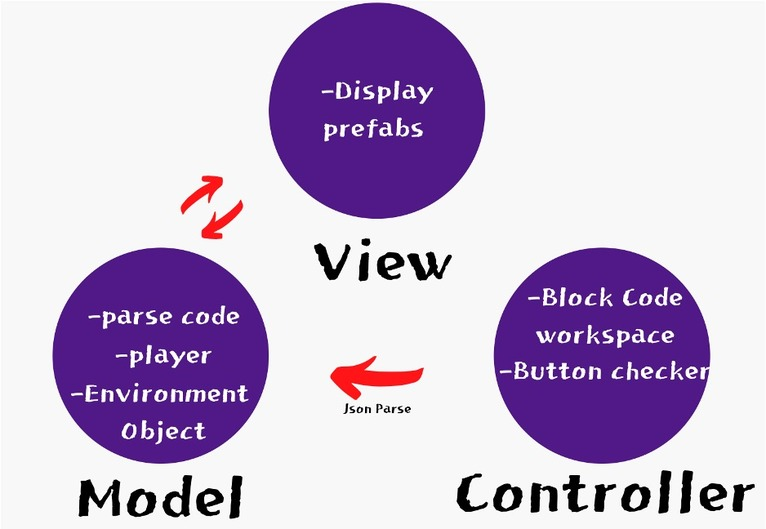
\includegraphics{pic/pic1.jpg}
\end{center}
\caption[Poem]{Design Pattern MVC}
\label{fig:walrus}
\end{figure}

\subsection{Model}
 ในส่วนของ Model จะเป็นการจัดการแปลงจาก Block Code ให้เป็น C\# เพื่อทำให้เกิด Event ต่างๆ เช่นการเดิน, การหมุน
 และการกระโดด เป็นต้น โดยที่ Model จะรับBlock Code มาจาก Controller ในรูปของ JSON
 และจะทำการแปลงเป็น C\# เพื่อสั่งให้ view แสดงผลต่างๆ ส่วนของ Model จะอยู่ใน Unity
 เป็นตัวกลางในการสื่อสารระหว่าง View กับ Controller

\subsection{View}
View นั้นทำหน้าที่แค่แสดงผลโดยรับโค้ดคำสั่งมาจาก Model และทำการแสดงผล จากนั้นจะทำการ
ส่งค่าคืน เพื่อบอก Model ว่าแสดงผลตามเสร็จตามคำสั่งนั้นแล้ว ในส่วนของ View นั้นจะอยู่ใน
Unity เช่นกัน เพราะ View ใช้แสดงผลกราฟฟิกของ Unity ที่ผู้พัฒนาได้สร้างเอาไว้ เช่น prefabs(รูปแบบสำเร็จ) ต่างๆ

\subsection{Controller}
Controller จะอยู่ทั้ง 2 ฝั่ง คือทั้ง Unity และ WebView โดย Controller ฝั่งหน้าเว็ปจะเป็นการรอให้ผู้ใช้
ลากวางตัว Block Code และเมื่อผู้ใช้กดรัน Controller ฝั่งหน้าเว็ปจะทำการแปลง Block Code ให้เป็น Object 
ในรูปของ JSON และจะถูกนำส่งไปให้ Controller ฝั่ง Unity หลักจากนั้น Controller ฝั่ง Unity จะทำการ
ประมวลผลและแปลงเป็น Object ที่ Unity สามารถอ่านได้เพื่อส่งต่อไปให้ Model

\section{WebView}
ตัวหน้าเว็ปทำขึ้นมาเพื่อนำ Google Blockly ไปใส่ใน panel ของ Unity เพระาเดิมที Unity ไม่สามารถสร้าง Object ที่หน้าตาและรวมไปถึง function ที่เหมือนกับ Google Blockly ได้ ทางผู้พัฒนาเลยสร้างหน้าเว็ปเข้ามาเพื่อนำไปใส่ใน 
panel ของ Unity ที่ใช้ในการแสดงผล Block Code
\begin{figure}
\begin{center}
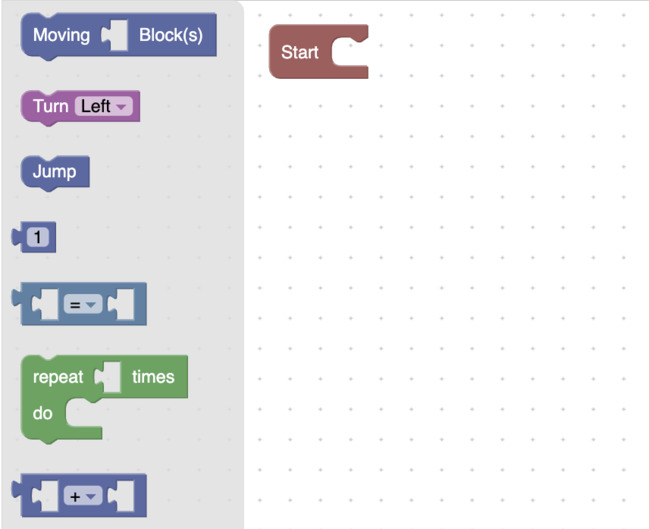
\includegraphics{pic/block1.jpg}
\end{center}
\caption[Poem]{Google Blockly}
\label{fig:walrus}
\end{figure}
